\section{Planned state of the application} The main reason of creating a new application instead of refactoring the current one is a change of the application's architecture. A new modernized architectural design of the BI-DBS portal was composed by Ing. Andrii Plyskach in his thesis. We are aiming to correct all the mistakes made in the current application. It is essential to ascertain that we have chosen the right stack of technologies according to the newly chosen architecture.

\subsection{Architecture}
Microservices architectural pattern is based on the concept of a series of loosely-coupled services. They can be developed using different technologies and deployed independently. It is more complex architecture then a standard monolithic one. 

\paragraph*{Advantages:}
\begin{itemize}
  \item Code readability. When services are not strongly dependent the code appears to be better structured and easier for understanding and that is the crustal benefit for the BI-DBS portal.
  
  \item Independency in choosing a stack of technologies. Microservices can be developed using different technologies which can be chosen according to the each microservice functionallity without affecting other microservices.
  
  \item Faster deployments. Since all microservices can be deployed independently the deploying part is much smaller and the time for deploying one service is rather shorter.

  \item Fault tolerance. Because of loose-coupling failing one of the microservices will not bring down the entire application.
\end{itemize}

\paragraph*{Disadvantages:}
\begin{itemize}
  \item Difficult debugging and testing. Each service needs to be first tested separately and only then as one unit. Besides it is more difficult to track down errors.

  \item DevOps required. To benefit from the fast deployment it should be configured and maintained. It requires the knowledge of development operations. DevOps concepts and configuration of automated deployment are described in the second chapter.

  \item Longer development time and limited reuse of code. Microservices need to be managed separately, therefore it requires more time.
\end{itemize}

\begin{figure}[hp]
\centering
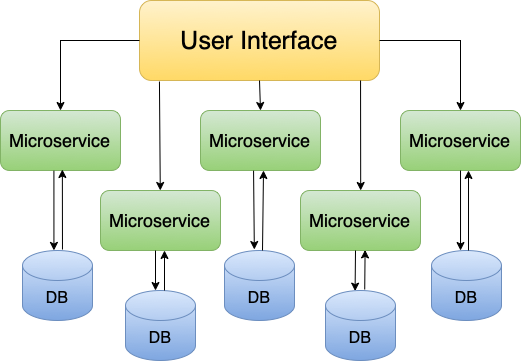
\includegraphics[scale=0.67]{../png/microservices.png}
\caption{Microservice architecture}\label{picture:mvp}
\end{figure}


%%%%%%%%%%%%%%%%%%%%%%%%%%%%%%%%%%%%%%%%%%%%%%%%%%%%%%%%%%%%%%%%%%%%%%%


\subsection{Technologies}

\paragraph*{PHP.} Since version 5.0, PHP supports object-oriented functionality. PHP is easy to learn, flexible, and supports all required functionalities for our application. It is used in a new project for a domain and business logic on the backend for API implementation.

\paragraph*{Symfony.} Symfony is a powerful back-end framework for creating complex applications which consists of reusable components. It is constantly growing and improving, besides it has a strong community. It is easy to learn and has a well-written documentation.


\paragraph*{Vue 3.} When the decision to create new BI-DBS portal has not yet been made its frontend was getting modernized with rewritting components to Vue.js version 2. In the new project it was chosen to carry on using Vue.js framework but use a new version 3. This version comes with some certain advantages for the application.

\paragraph*{New features:}
\begin{itemize}
  \item Composition API. Composition API is a set of APIs that allow us to create Vue components by importing functions rather than defining options. Mainly it benefits our project better code organization thus makes a project better structured and code easier to read. Moreover, Composition API enables efficient logic reuse.
  
   \item Vite. Vite is fontend build tool from the cratetor of Vue.js - Evan You. It is module bundler which is built on top of webpack, it will bundle the entire project on startup, hot reloads, and compilation. The primary purpose for the change is for speed. The server starts instantly since it uses native browser support for JavaScript modules.

   \item Increased rendering performance.

\end{itemize}

\paragraph*{Quasar} Quasar is a web framework based on Vue.js. It provides us with ready-to-use components which are customizable and easy-extendable. Moreover, it makes the application less vulnerable to XSS attacks due to its escaping feature. When using Quasar, developers do not need deep knowledge of CSS and scripting languages to build a good-looking  and responsive application. Besides, it is suitable for developing single-page applications(SPA).

\paragraph*{Typescript} Typescript is based on JavaScript which is dynamically typed. TypeScript has an additional syntax which makes it statically typed. That has advantages in catching errors during development. It also gives a code more structure and makes it predictable. Typescript is more suitable for big applications than JavaScript. For our project, it is crucial to write code that will be easy to read.


%%%%%%%%%%%%%%%%%%%%%%%%%%%%%%%%%%%%%%%%%%%%%%%%%%%%%%%%%%%%%%%%


\subsection{Potential problems and possible solutions}